\documentclass[a4paper]{article}

\usepackage[latin1]{inputenc}
\usepackage{amssymb}
\usepackage{framed}
\usepackage{graphicx}
\usepackage{subcaption}



\setlength{\parindent}{0pt}
\setlength{\parskip}{3ex}

\begin{document}

\begin{center}
  {\large Artificial Neural Networks and Deep Architectures, DD2437}\\
  \vspace{7mm}
  {\huge Short report on lab assignment 1\\[1ex]}
  {\Large Classification with a single-layer perceptron}\\
  \vspace{8mm}  
  {\Large Hasan Alzubeidi, Rakin Ali and Steinar Logi \\}
  \vspace{4mm}
  {\large January 22, 2024 \\}
\end{center}

\section{Main objectives and scope of the assignment \normalsize}
The main objective with this assignment is to familiarize ourselves with the perceptron learning rule and the delta learning rule along with batch versus sequential learning method. 
Our major goals in the assignment were  
\begin{itemize}
\item Implement and explore the perceptron learning rule for simple classification tasks
\item Explore how the perceptron and delta learning rule performs on linearly separable data compare to a dataset that is not linearly separable
\item Explore how the bias affects the convergence of the delta learning algorithm
\end{itemize}

This assignment was scoped on the delta and perceptron learning rule. For the delta rule we used batch learning and sequential learning; for perceptron learning rule, we only used sequential learning. The limitations was that we didn't test around a lot with different learning rates, we simply one the ones that seemed reasonable. 

\section{Methods} This lab was conducted three separate times as we did not collaborate when writing the code. We all did the code separately then compared our results. The code was written in Jupyter notebook and regular python v3.9 file. We all drew more or less the same conclusions based on our results however got different graphs. Numpy function and matplot were the only libraries used.  \\

\section{Results and discussion}
\subsection{Classification with a single-layer perceptron}
\textbf{Perceptron versus Delta Rule Learning: }In this Section we compared two learning algorithms with a single perception. The algorithms compared were delta rule and perception learning. From the lectures we learned that perceptron learning converges to the "first best solution" it finds however that result does not generalize well compared to delta rule. This is evident in figure \ref{fig:Decision Boundary} as the boundary line generalizes better. Regarding convergence, delta rule converges faster as a lot less iterations were needed. 
\begin{figure}[htb]
    \centering
    \begin{subfigure}{0.4\textwidth}
        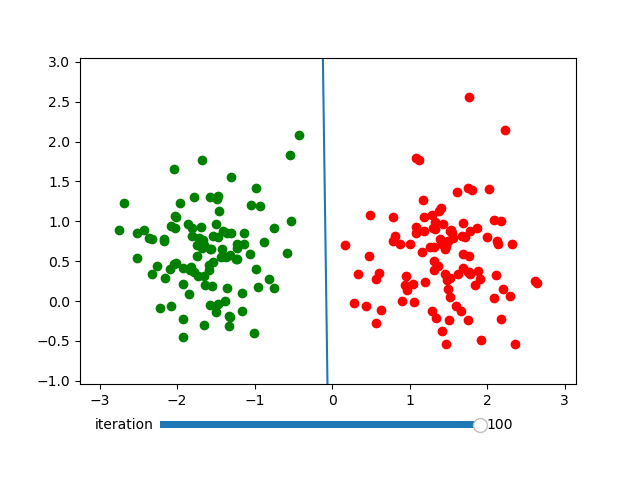
\includegraphics[width=\textwidth]{Labs/Lab 1/Lab 1a/Results/Delta-linear-seperable.png}
        \caption{Delta rule}
        \label{fig:Delta Rule}
    \end{subfigure}
    \hfill
    \begin{subfigure}{0.4\textwidth}
        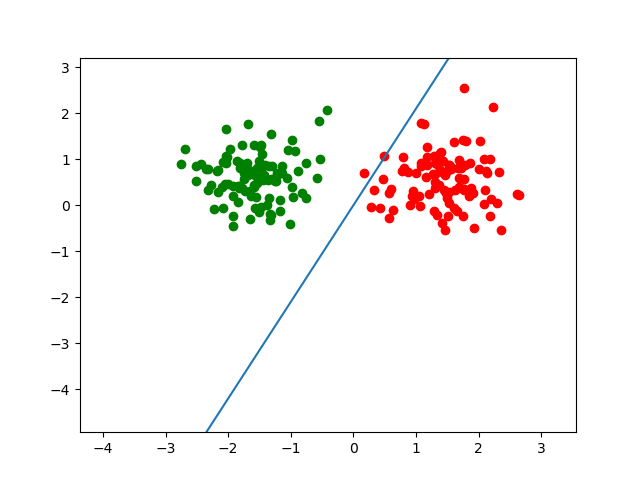
\includegraphics[width=\textwidth]{Labs/Lab 1/Lab 1a/Results/perceptron-linearly-seperable.png}
        \caption{Perceptron rule}
        \label{fig:Perceptron}
    \end{subfigure}
    \caption{Decision Boundary for Delta rule and Perceptron Rule}
    \label{fig:Decision Boundary}
\end{figure}\\
\textbf{Removing Bias check: }we also removed the bias to check how well delta rule converges. This can be seen in figure \ref{fig:DeltaRule-NoBias}
\begin{figure}[htb]
    \centering
    \begin{subfigure}{0.4\textwidth}
        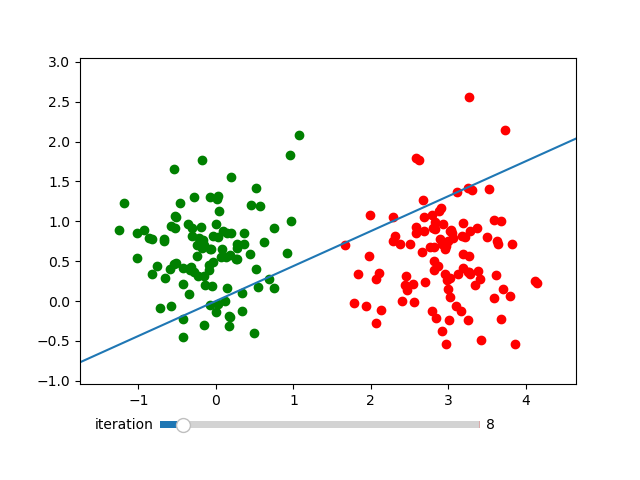
\includegraphics[width=\textwidth]{Labs/Lab 1/Lab 1a/Results/Delta-linear-seperable-NO-BIAS.png}
        \caption{Delta rule with 8 iterations}
        \label{fig:Delta Rule without bias, iteration 8}
    \end{subfigure}
    \hfill
    \begin{subfigure}{0.4\textwidth}
        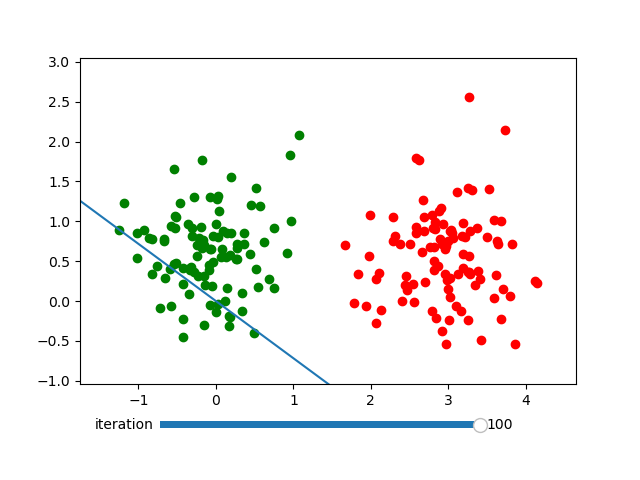
\includegraphics[width=\textwidth]{Labs/Lab 1/Lab 1a/Results/Delta-linear-seperable-NO-BIAS-ITERATION100.png}
        \caption{Delta rule with 100 iterations}
        \label{fig:Perceptron}
    \end{subfigure}
    \caption{Decision Boundary for Delta rule without bias }
    \label{fig:DeltaRule-NoBias}
\end{figure}
The decision boundary passes through origo regardless if it is not the optimal solution. The slope changes to become as optimal as possible. The bias simply changes the "starting" position of the slope which makes it easier to find the optimal decision boundary. 

\newpage
\textbf{Batch versus sequential learning:} Lastly we compared sequential versus batch learning. They converge to the same result however batch makes the changes faster after each iteration. It "stores" all the changes after each epoch then adds the changes while sequential ad
\begin{figure}[htb]
    \centering
    \begin{subfigure}{0.4\textwidth}
        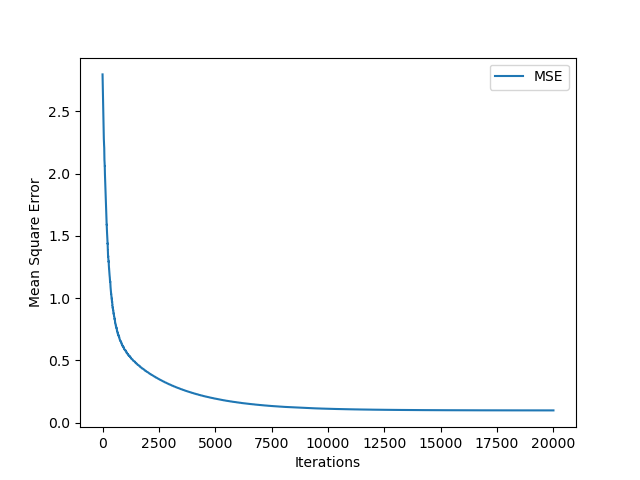
\includegraphics[width=\textwidth]{Labs/Lab 1/Lab 1a/Results/delta-linear-seperable-bias-sequential.png}
        \caption{Delta rule with sequential learning}
        \label{fig:Delta Rule with sequential learning}
    \end{subfigure}
    \hfill
    \begin{subfigure}{0.4\textwidth}
        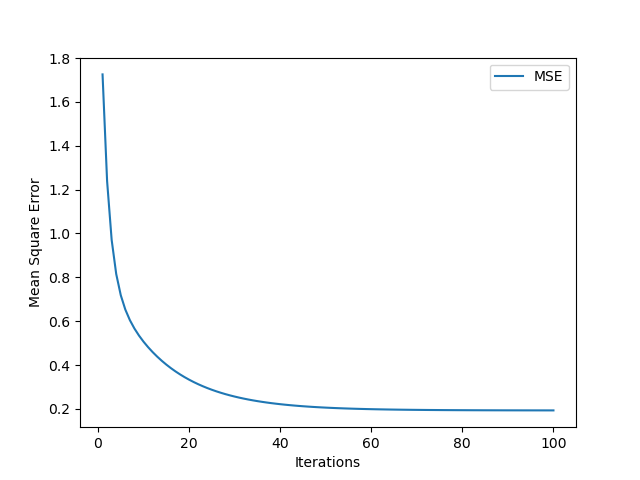
\includegraphics[width=\textwidth]{Labs/Lab 1/Lab 1a/Results/delta-linear-seperable-bias-BATCH.png}
        \caption{Delta rule with batch learning}
        \label{fig:DeltaRule with batch learning}
    \end{subfigure}
    \caption{Mean square error comparison of online and sequential learning}
    \label{fig:DeltaRule-NoBias}
\end{figure}


\subsection{Classification of data that are not linearly separable}
\textbf{Perceptron training:} We created a dataset that is not linearly separable by using the same method as in the assignments above, moving the means of the two clusters closer together. First we tried fitting the single layer Perceptron using the Percepton learning algorithm. We expected that this would not work since it is only guaranteed that it converges if the dataset is linearly separable. Our simulations confirmed this. We tried fitting this Perceptron using the Perceptron learning rule. We calculated the mean square error in the same way as is done when using the Delta learning to get a glimpse into the error of the model. The model does not converge.

\begin{figure}[htb]
    \centering
    \begin{subfigure}{0.4\textwidth}
         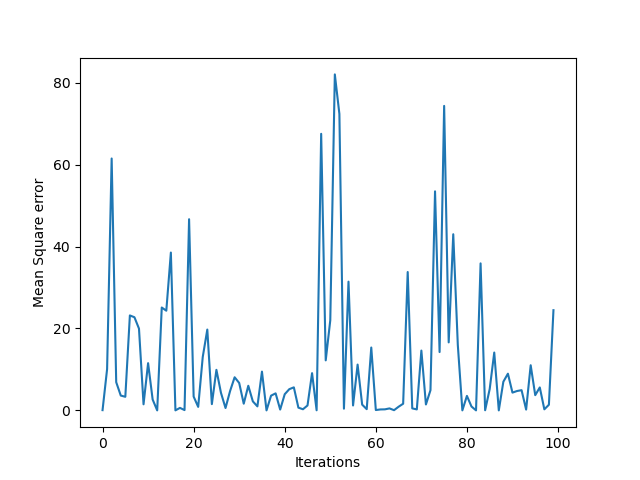
\includegraphics[width=\textwidth]{Labs/Lab 1/Lab 1a/Results/perceptron-NON_SEPERABLE_training_errorRate(rakin-modifed).png}
        \caption{Training error when using Perceptron}
        \label{fig:Perceptron-training-error}
    \end{subfigure}
    \hfill
    \begin{subfigure}{0.4\textwidth}
        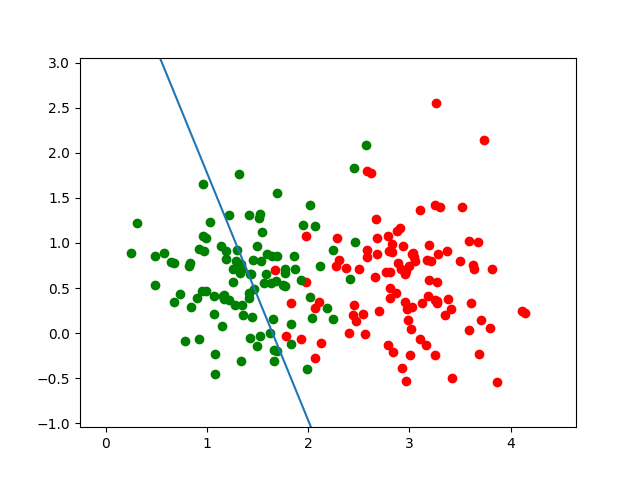
\includegraphics[width=\textwidth]{Labs/Lab 1/Lab 1a/Results/perceptron-decision-boundary-not-separable.png}
        \caption{Decision boundary}
        \label{fig:decision-boundary}
    \end{subfigure}
    \caption{Error rate and Decision boundary of Perceptron Learning}
\end{figure}

The training error never reaches a point where it is stable. This makes sense since there will always be a point that is misclassified. When the training algorithm reaches that point it moves the boundary in a such a way that it will be on the correct side of the boundary. That will make another point misclassified and therefore this boundary will always keep on moving to make the current point correctly classified. An illustration of this can be seen below.

\begin{figure}[htb]
    \centering
    \begin{subfigure}{0.3\textwidth}
        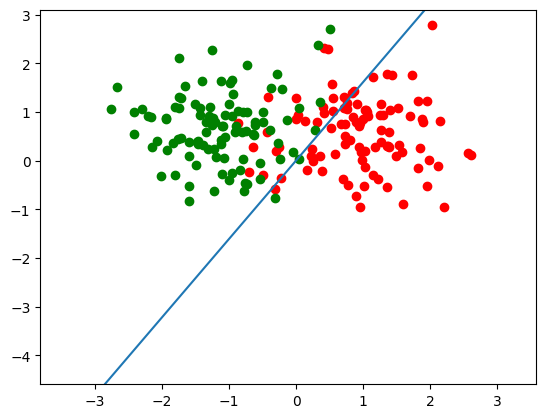
\includegraphics[width=\textwidth]{Labs/Lab 1/Lab 1a/Results/p_non_linear10000.png}
        \caption{Decision boundary after 10000 iterations}
        \label{fig:Decision-boundary-not-linearly-separable}
    \end{subfigure}
    \hfill
    \begin{subfigure}{0.3\textwidth}
        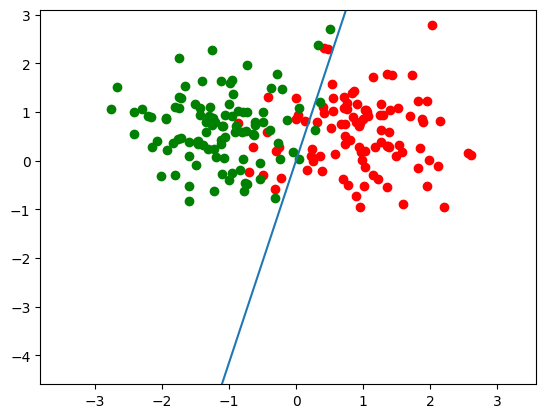
\includegraphics[width=\textwidth]{Labs/Lab 1/Lab 1a/Results/p_non_linear11000.png}
        \caption{Decision boundary after 11000 iterations}
        \label{fig:Decision-boundary-not-linearly-separable}
    \end{subfigure}
    \caption{Two different decision boundaries obtained with the perceptron learning}
\end{figure}

\textbf{Delta Rule Training: }We used a single layer Perceptron, trained using the Delta learning rule to classify the same dataset seen in figure. We expected the learning algorithm to converge when using an appropriate learning rate. The algorithm did converge and we obtained the decision boundary shown in figure \ref{fig:6}. The other picture shows how the training error developed through the training. It decreases fast in the beginning until it reaches convergence. 
\begin{figure}[htb]
    \centering
    \begin{subfigure}{0.4\textwidth}
        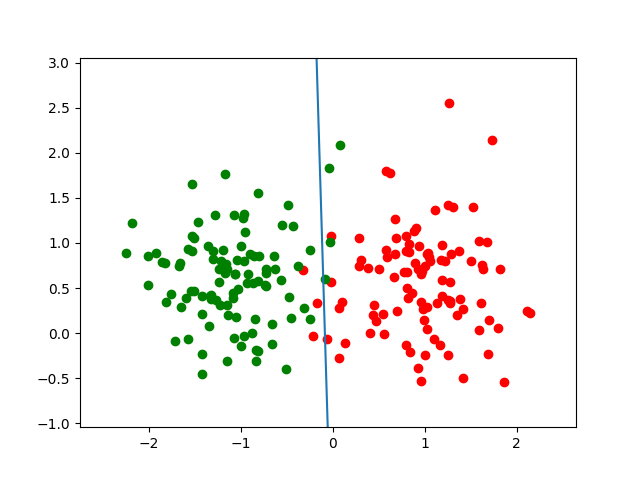
\includegraphics[width=\textwidth]{Labs/Lab 1/Lab 1a/Results/decicion-boundary-not-separable.png}
        \caption{Decision boundary on data set that is not linearly separable with Delta rule}
        \label{fig:Decision-boundary-not-linearly-separable}
    \end{subfigure}
    \hfill
    \begin{subfigure}{0.4\textwidth}
        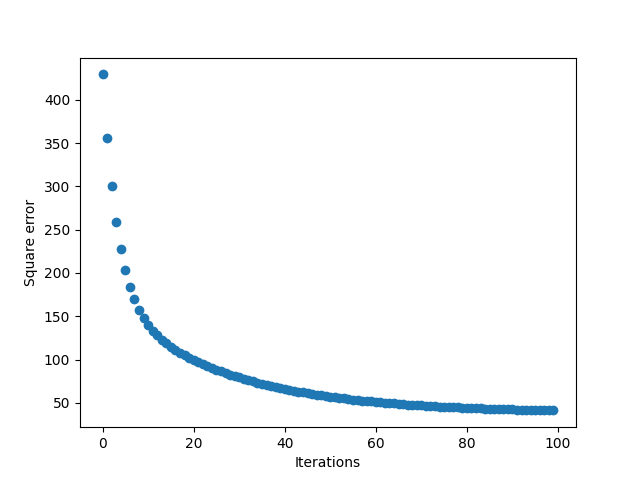
\includegraphics[width=\textwidth]{Labs/Lab 1/Lab 1a/Results/error-convergance.png}
        \caption{Delta rule with 100 iterations}
        \label{fig:Error-convergance}
    \end{subfigure}
    \caption{Decision boundary and MSE using the delta rule}
    \label{fig:6}
\end{figure}
We created another kind of dataset that is not linearly separable. It was created in such a way that the data belonging to one of the classes was generated the same way as before, i.e. a multivariate Gaussian with a single mean and variance. The other class was created in such a way that half of the data points belonging to that class were generated using the mean $mA$ and the other half generated using the mean $-mA$. We then trained the perceptron using the delta learning rule and obtained the decision boundary shown in figure \ref{fig:new-dataset}. We can see that the delta learning rule does converge but the mean square error is a lot higher than for the previous data sets. And the accuracy obtained on this data set is 0.775
\begin{figure}[htb]
    \centering
    \begin{subfigure}{0.4\textwidth}
        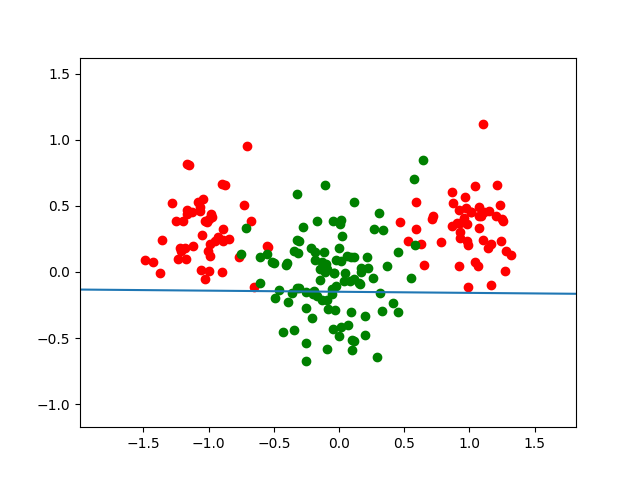
\includegraphics[width=\textwidth]{Labs/Lab 1/Lab 1a/Results/new-data.png}
        \caption{The new data set}
        \label{fig:new-dataset}
    \end{subfigure}
    \hfill
    \begin{subfigure}{0.4\textwidth}
        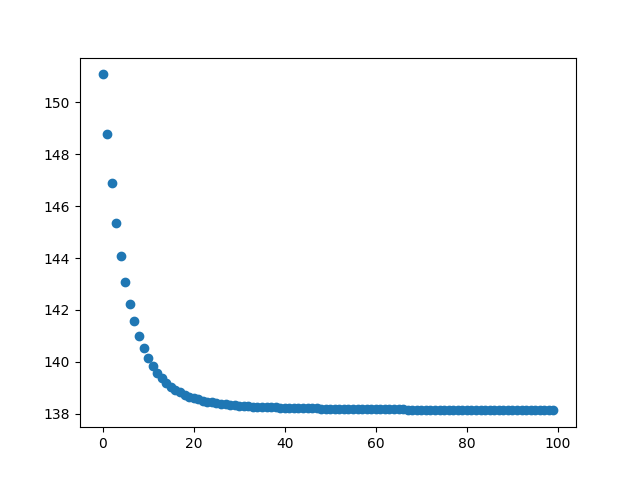
\includegraphics[width=\textwidth]{Labs/Lab 1/Lab 1a/Results/new-data-convergance.png}
        \caption{Delta rule with 100 iterations}
        \label{fig:new-data-convergance}
    \end{subfigure}
    \caption{Decision boundary and convergance}
    \label{fig:8}
\end{figure}

We then tried a few ways to exclude data from the set of data that the model is trained on. We used the data that was left as unseen data to test the accuracy. The scenarios are the following:
\begin{enumerate}
    \item Random 25\% from each class
    \item Random 50\% from class A
    \item Random 50\% from class B
    \item 20\% from a subset of classA for which classA(1,:)<0 and 80\% from a
subset of classA for which classA(1,:)>0
\end{enumerate}

The decision boundaries obtained for each of these scenarios can be seen in figure \ref{fig:9}.

\begin{figure}[htb]
    \centering
    \begin{subfigure}{0.4\textwidth}
        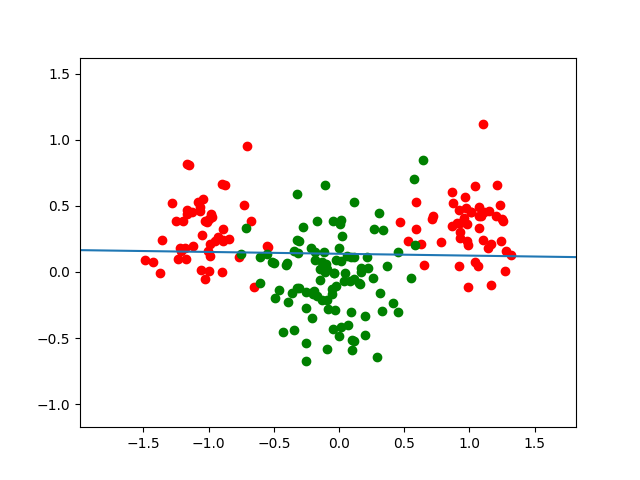
\includegraphics[width=\textwidth]{Labs/Lab 1/Lab 1a/Results/scenario1.png}
        \caption{Scenario 1}
        \label{fig:scenario-1}
    \end{subfigure}
    \hfill
    \begin{subfigure}{0.4\textwidth}
        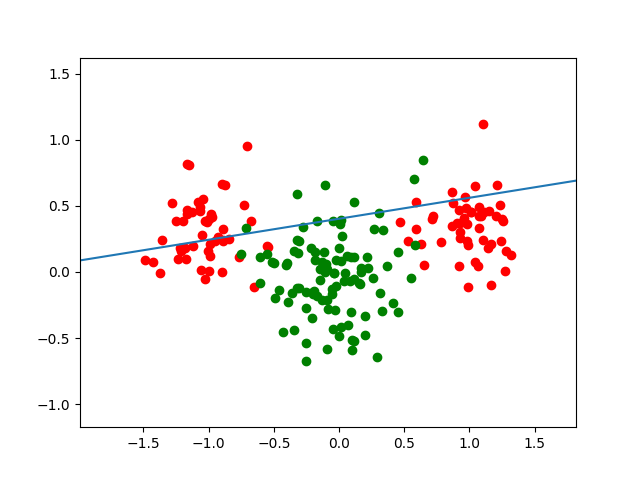
\includegraphics[width=\textwidth]{Labs/Lab 1/Lab 1a/Results/scenario2.png}
        \caption{Scenario 2}
        \label{fig:scenario-2}
    \end{subfigure}
     \begin{subfigure}{0.4\textwidth}
        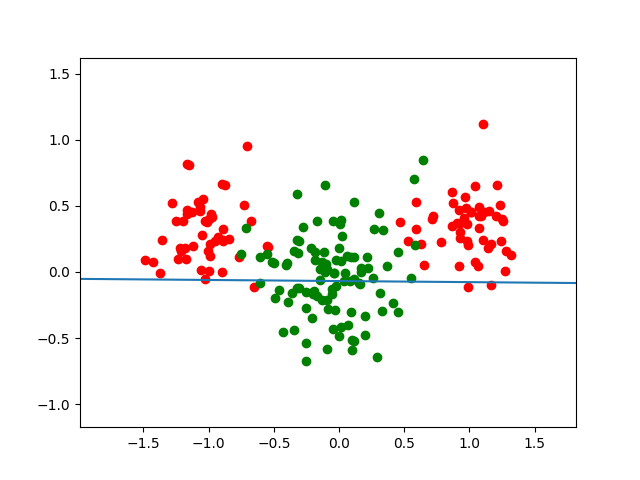
\includegraphics[width=\textwidth]{Labs/Lab 1/Lab 1a/Results/scenario3.png}
        \caption{Scenario 3}
        \label{fig:scenario-3}
    \end{subfigure}
    \hfill
    \begin{subfigure}{0.4\textwidth}
        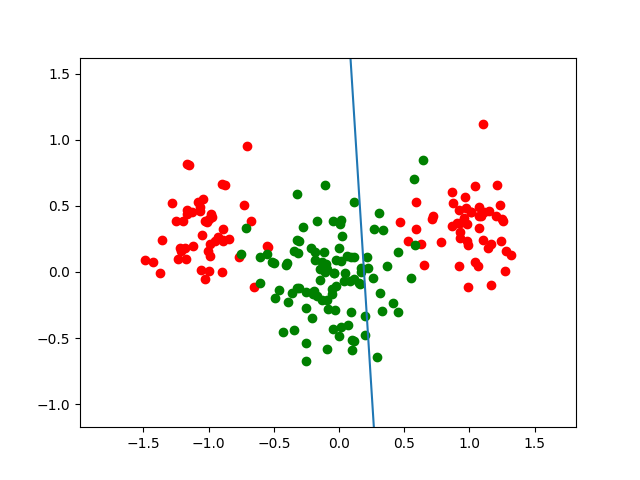
\includegraphics[width=\textwidth]{Labs/Lab 1/Lab 1a/Results/scenario4.png}
        \caption{Scenario 4}
        \label{fig:scenario-4}
    \end{subfigure}
    \caption{Decision boundaries with different data removed}
    \label{fig:9}
\end{figure}

The accuracy of the training data in scenario 1 was 81\% for class A and 81\% for class B. Which is not much worse than when none of the data was removed. The accuracy on the test data was slightly worse but not significantly or 80\% for class A and 72\% for class B. This makes sense since the data that is removed before training is removed uniformly from each class so the 
\\
Scenario 2 gave us much more interesting results. The accuracy on the training set was only 0.36 for class A and 0.93 for class B. The accuracy for the test set was 28\% for class A. Since the training set is unbalanced the wrongly classified points in class A do not contribute as much to the loss function that we are minimizing. Therefore the accuracy is much lower for class A.
\\
Scenario 3 was very similar to scenario 2 but the other way around. The perceptron classified 97\% of the points in class A correctly but only 28\% of the test set points in class B.\\
We found scenario 4 to be the most interesting one. The training accuracy was 76\% for class A and 96\% for class B. But the test accuracy was only 18\% for class A. since we removed most of the points in the right cluster of points belonging to class A and only a few from the left cluster, the perceptron benefits from classifying more points from class B correctly. As can be seen in the figure above the classification boundary is a bit to the right of the center of cluster B.

\section{Final remarks} 
In this lab we implement the theoretical concepts practically. A single perception was created and trained using two learning algorithms being delta rule and perception training. What we learned was:
\begin{itemize}
    \item The bias term matters. Removing it affects the decision significantly and can decrease the performance of the perception
    \item Initialization matters. We had to find different learning rules and continuously asked ourselves \textit{is this result reasonable?} Many times it was due to the learning rate being too high or low, too few iterations and other stuff that mattered. 
    \item Delta rule in most cases seems to be the better option. It produces a better decision boundary, converges somewhat faster than perception learning and generalizes better. 
    \item Sequential versus batch should not matter much when dealing with small datasets. From our findings on this lab, we did not notice a significant difference in terms of results other than the iterations were much higher for sequential. For large datasets, batch would have speed up computations significantly. 
\end{itemize}


\end{document}
